\documentclass[11pt, fontset = fandol]{ctexbeamer}
\usepackage{fontspec}
\usepackage{listings}

\usefonttheme[onlymath]{serif}
\setmonofont{Consolas}

\lstset{
  basicstyle={
    \color{black}
    \fontspec{Consolas}
  },
  keywordstyle={
    \color{blue}
    \fontspec{Consolas}
  },
  numberstyle={
    \color{gray}
    \fontspec{Consolas}
    \small
  },
  rulecolor=\color{blue},
  frame=single,
  morekeywords={Sample, Input, Output},
}

\usetheme{CambridgeUS}
% \usetheme{PaloAlto}
\usecolortheme{crane}

\title{\texttt{NNSZCP-2023} 题解}
\author{南宁三中 01 社}
\begin{document}
\begin{frame}
  \maketitle
\end{frame}
\section{A 欢迎光临}
\subsection{简明题解}
\begin{frame}[fragile]
  \pause
  \begin{block}{题意}
    给定字符串,查询子串有没有 \texttt{nnsz}。
    字符串长度 $\le 100$。
  \end{block}
  \pause
  签到题。\\
  \pause
  枚举相邻的字符判断是否为 \texttt{nnsz} 即可。\\
  \pause
  当然也可以用 KMP 做。\\
  \pause
  时间复杂度 $O(n)$。\\
  \begin{lstlisting}
print("yes" if "nnsz" in input() else "no")
  \end{lstlisting}
\end{frame}

\section{B 反应原理}
\subsection{简明题解}
\begin{frame}[fragile]
  \pause
  \begin{block}{题意}
    给定 $n$ 和长为 $n+1$ 的序列 $a$,求相邻两项最大差值、最大值。\\
    保证 $1 \le n \le 3 \times 10^5$。

  \end{block}
  按题意模拟即可。\\
  \pause
  注意序列的长为 $n+1$。\\
  \pause
  \begin{lstlisting}
n = int(input())
a = [int(i) for i in input().split()]
print(max(a))
b = [a[i + 1] - a[i] for i in range(n)]
print(max(b))
  \end{lstlisting}
\end{frame}

\section{C 暮光闪闪}
\subsection{题意}
\begin{frame}
  \begin{block}{题意}
  	$ n $ 栋建筑物,每一栋建筑物的高度为 $ h_i $。\\
  	$ m $ 匹天马中,对于第 $ i $ 匹天马,其飞行的高度为 $ s_i $。\\
  	对两座建筑 $i, j$,第 $k$ 匹天马能够在这两座建筑之间飞行,当且仅当 $\mid h_i - h_j \mid \le s_k$。\\
  	对于每一匹天马,求其最多能够在多少对建筑之间穿梭?\\
  	保证 $ 1 \le m \le 10^5$,$1 \le n \le 2 \times 10^3 $。
  \end{block}
\end{frame}

\subsection{简要题意}

\begin{frame}
\pause
对于 Subtask 0:对于每匹天马,枚举每一对建筑,并判断它是否能在该对建筑之间穿梭。时间复杂度为 $ \mathcal{O} \left(n^2m\right) $。\\
\pause
对于 Subtask 1:由 $ s_i > 0 $ 可知,每一匹天马均可在建筑中任意穿梭,故答案为 $ \frac{n(n - 1)}{2} $。\\
\pause
对于 Subtask 2:\\
\pause
预处理每对建筑之间的高度差,并将其升序排序。对于每匹天马,在高度差数组中通过二分查找得到答案。\\
\pause
预处理高度差并排序的时间复杂度为 $ \mathcal{O} \left(n^2 \log{n^2} \right) $,进行 $ m $ 次二分查找的时间复杂度为 $ \mathcal{O} \left(m \log{n^2} \right) $,故总时间复杂度为 $ \mathcal{O} \left(\left(n^2 + m\right) \log{n^2} \right) $,可以通过。\\
\pause
有更优的做法,但这是 C。
\end{frame}

\section{D 中考报名}

\subsection{题意}
\begin{frame}
  \begin{block}{题意}
    按照一定规则对进行考生进行排名。\\
    详细内容见题面。保证 $1 \le n \le {10} ^5$。
  \end{block}
\end{frame}

\subsection{简要题解}
\begin{frame}
	\pause
	本题是模拟题。减小编码难度、减少码量从而快速解决本题,才能拥有更多的时间解决后面的题目。\\
	\pause
	本题 \texttt{C++} 标程仅约 700 Byte,\texttt{Python} 标程仅约 400 Byte,它z们都用到了以下优化技巧来减小码量。\\
	\pause
	\begin{itemize}
		\item 使用 \texttt{tuple} 而非 \texttt{struct} 或 \texttt{class} 表示考生。
		\pause
		\item 运用位运算技巧,仅用一个整数即可表示考生各科 $ \texttt{A+} $ 情况。
		\pause
	\end{itemize}
	运用位运算技巧将考生各科 $ \texttt{A+} $ 情况压缩成一个整数,即可以方便地在 \texttt{tuple} 中存储考生的数据,又可以通过直接比较整数的大小来分出成绩的优劣。\\
	\pause
	而且,\texttt{tuple} 自带关键字比较功能,我们无需重载运算符或手写 \texttt{cmp()} 函数,进一步减小了码量。\\
\end{frame}

\section{E 填数游戏}
\subsection{题意}
\begin{frame}
  \begin{block}{题意}
  	构造一个 $n \times n$ 的矩阵,每个元素都 $\in \left[0, k\right]$,使得任意选择不在同行或同列的数直到无法选择后,将它们求和得到 $k$,或判断无解。\\
  	多组数据,$1 \le T \le 10$,$1 \le n \le 500$,$1 \le k \le {10}^9$。\\
  \end{block}
\end{frame}

\subsection{简要题解}
\begin{frame}
	\pause
	可以先考虑无解的情况,构造一个从 $0$ 开始一直加到 $n^2-1$ 的矩阵,这显然是最小的合法矩阵。\\
	\pause
	对其按题意的操作求和后的值为 $s=\frac{(n+1)n(n-1)}{2}$ ,如果所给的 $k < s$,就是无解的情况,因为我们无法构造出比这个还小的矩阵,否则就会出现重复的元素。\\
	\pause
	如果你只输出 -1 ,是一分也没有的。\\
\end{frame}

\begin{frame}
	\pause
	那么要怎么构造呢?\\
	\pause
	我们现在已经有一个最小的合法矩阵了,其实只要在这个基础上加一加就好了。\\
	\pause
	具体的,只要把最大那行 $l$(从 $n^2-1-n$ 到 $n^2-1$)都加上 $(k-s)$ 就好了,因为每行只会选出一个元素, $l$ 中元素也一定会被选到一个,就会使得 $s\leftarrow s+(k-s)$,在最大一行加是为了避免元素重复,于是就做完了。\\
	\pause
	当然其实不只这一种构造方法,但只要构造出的矩阵相邻两列中每一行元素的差都相等,就可以使得任意选出来的结果都一样,然后再使得结果与 $k$ 相等即可。\\
\end{frame}

\section{F 初生几何}
\subsection{题意}
\begin{frame}
  \begin{block}{题意}
    如图,在平面直角坐标系中,抛物线 $ y = x\left(k - x\right) $ 与直线 $ y = -1 $ 相交。抛物线与 $ x $ 轴的另一个交点为 $\mathrm{A}$。设\textbf{线段} $\mathrm{OA}$ 上存在一动点 $\mathrm{P}$,过点 $\mathrm{P}$ 作 $y$ 轴的平行线交抛物线于点 $\mathrm{B}$,交直线 $y = -1$ 于点 $\mathrm{C}$。\\
    试求 $\mathrm{OB}^2 + \mathrm{AC}^2$ 的最大值。
  \end{block}
\end{frame}

\subsection{简易题解}
\begin{frame}
  \pause
  我会猜想!\\
  \pause
  注意到:$P\left(\frac{365}{508}, 0\right)$ 时恰有:
  $$
  \begin{aligned}
    \mathrm{OB}^2 + \mathrm{AC}^2 &= \frac{17,748,900,625}{66,597,028,096} + \frac{133,225}{129,032} + 1\\
    &= \frac{153,107,081,521}{66,597,028,096} \approx 2.29900771698543729578
  \end{aligned}
  $$
  因此 $P$ 必定为 $(\frac{k}{2}, 0)$。\\

\end{frame}

\subsection{证明}
\begin{frame}
  \pause

  \begin{figure}[H]
    \centering
    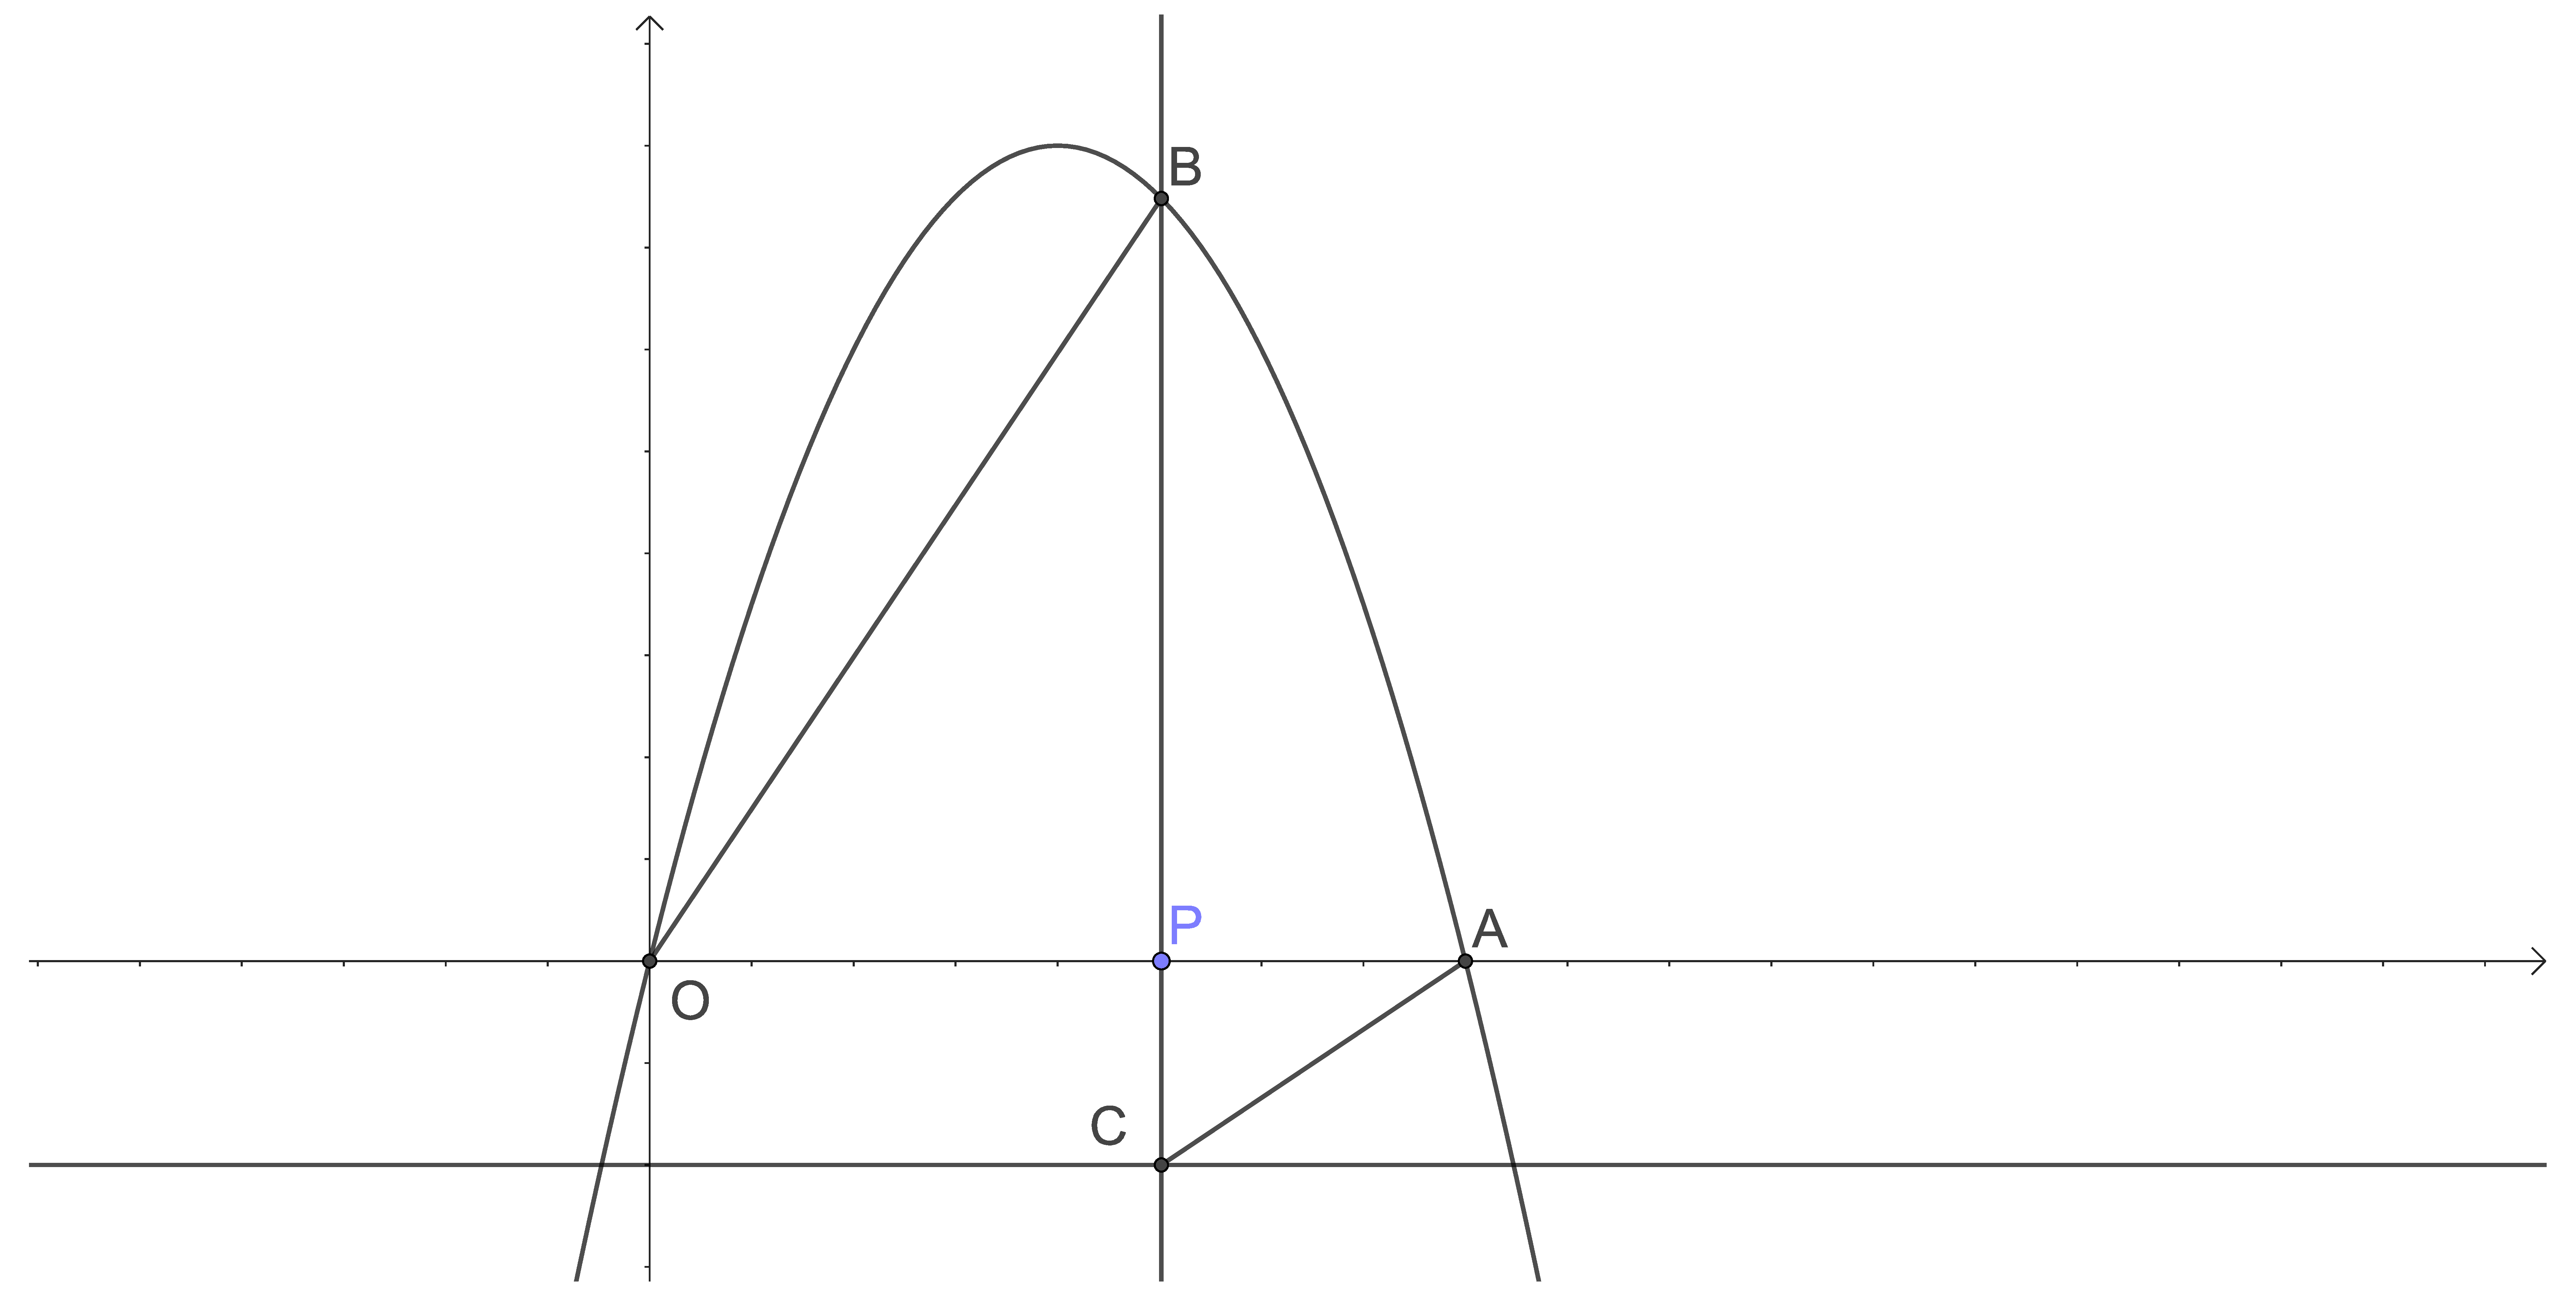
\includegraphics[scale=0.08]{pic.pdf}
  \end{figure}

  \pause

  由基本不等式可知当 $P$ 为中点时 $\mathrm{OP}^2 + \mathrm{AP}^2$ 取到最大,而由抛物线性质 $\mathrm{BP}^2$ 同时取到最大。

  std 直接计算了 $\mathrm{BC}^2$(不难证明是等价的)。

\end{frame}

\section{G 排序算法}
\subsection{题意}
\begin{frame}[fragile]
  \begin{block}{题意}

    判断排序算法的正确性,并求这个排序算法的交换次数。

    \begin{lstlisting}
for (int i = 1; i <= n; ++i) {
  for (int j = 1; j <= n; ++j) {
    if (a[i] < a[j]) {
      std::swap(a[i], a[j]);
    }
  }
}
    \end{lstlisting}

    保证 $1 \le n \le 2 \times {10}^5$。
  \end{block}
\end{frame}

\subsection{算法 0}
\begin{frame}[fragile]
  我会模拟!\\
  \pause
  模拟这个过程并判断序列是否有序。\\
  \pause
  时间复杂度 $O(n^2)$。\\
  \pause
  期望通过 Subtask 0,得到 20 分。\\
  \pause

  \begin{lstlisting}
int count = 0;
for (int i = 1; i <= n; ++i) {
  for (int j = 1; j <= n; ++j) {
    if (a[i] < a[j]) {
      std::swap(a[i], a[j]), ++count;
    }
  }
}
std::cout << count << '\n';
  \end{lstlisting}

\end{frame}

\subsection{算法 1}

\begin{frame}[fragile]
  我会思考性质!\\
  \pause
  归纳法容易证明算法正确性(详见下发题解)。\\
  \pause
  \begin{block}{性质}
    除了第 $ 1 $ 轮外层循环,每轮外层循环对答案的贡献为序列 $ \{ a_1, a_2, a_{i - 1} \} $ 中比 $ a_i $ 大的\textbf{不同}元素的个数。
  \end{block}
  \pause
  朴素处理第 $1$ 轮外层循环,再维护一个数据结构支持插入元素、查询大于某个元素的不同元素个数。\\
  \pause
  平衡树、线段树和树状数组即可。\\
  \pause
  时间复杂度 $O(n \log n)$。python 常数大只有树状数组能过。\\
  \pause
  期望通过所有子任务。

\end{frame}

\section{H 购买车券}
\subsection{题意}
\begin{frame}
  \begin{block}{题意}
    给定一棵无根树 $T$,每次删去一个叶子结点直至删空。\\
    对合法的操作序列计数,对 $998,244,353$ 取模。\\
    叶子结点的定义是度数不大于 $1$ 的结点。\\
    操作序列不同,当且仅当某一次删去的叶子不同。\\
    保证 $1 \le n \le 2 \times {10}^5$。\\
  \end{block}
\end{frame}

\subsection{算法 0}
\begin{frame}
  \pause
  我会枚举!\\
  \pause
  考虑在树上暴搜方案。\\
  \pause
  时间复杂度 $O(n!)$。\\
  \pause
  期望通过 Subtask 0。\\
\end{frame}

\subsection{算法 1}
\begin{frame}
  \pause
  我会性质!\\
  \pause
  由于整棵树是一条链,在删除前 $ n - 1 $ 个结点时,树上都恰好有 $ 2 $ 个叶子结点,故答案为 $ 2^{n - 1} $。\\
  \pause
  结合算法 0 期望通过 Subtask 0, 2。\\
\end{frame}

\subsection{算法 2}
\begin{frame}
  \pause
  我还会性质!\\
  \pause
  对一个菊花树,在删除第 $ i $ $\left(i \le n - 2\right) $ 个结点时,树上有 $ n - i $ 个叶子结点;在删除第 $ n - 1 $ 个结点时,树上有 $ 2 $ 个叶子结点。\\
  \pause
  故答案为:

  $$
  (n - 1) \times (n - 2) \times \cdots \times 3 \times 2 \times 2 \times 1 = (n - 1)! \times 2
  $$

  \pause
  结合算法 0, 1 期望通过 Subtask 0, 2, 3。\\
\end{frame}

\subsection{算法 3}
\begin{frame}
  \pause
  我会“動的計画法”!\\
  \pause
  思考对于一棵一般的树怎么做。\\
  \pause
  以结点 $x$ 为根,设 $f_u$ 代表将结点 $u$ 所在的子树删空的方案数。\\
  \pause
  不好转移,我们钦定 $u$ 是 $u$ 所在的子树最后删掉的点。\\
  \pause
  这样就比较好转移了。转移考虑 $u$ 的儿子 $v$:
  $$
  \begin{aligned}
    f_u &= \prod_{i} \left( f_{v_i} \cdot \binom{\sum_{j}^i s_j}{s_i} \right)\\
    &= \left(\prod_{i} f_{v_i} \right) \frac{(s_u - 1) !}{\prod_{{v_i}} (s_{v_i}!)}
  \end{aligned}
  $$
  其中 $s_u$ 代表以 $u$ 为根所在的子树大小。
  \pause
  令 $x = 1, 2, \cdots, n$ 跑这个 DP,对所有 $f_x$ 求和即为答案。\\
  时间复杂度为 $O\left(n^2\right)$。\\

  结合算法 1, 2 期望通过 Subtask 0, 1, 2, 3。\\
\end{frame}

\subsection{算法 4}
\begin{frame}
  \pause
  我会二次扫描!\\
  \pause
  考虑优化。\\
  \pause
  设 $g_u$ 代表将结点 $u$ 视为树根且最后删,删空整棵树的方案数。\\
  \pause
  转移依然考虑 $u$ 的儿子 $v$:\\
  $$
  \begin{aligned}
    g_v &= f_v \times \frac{g_u}{f_v \times \binom{n - 1}{n - s_v - 1}} \times \binom{n - 1}{s_v - 1}\\
    &= g_u \times \frac{\binom{n - 1}{s_v - 1}}{\binom{n - 1}{n - s_v - 1}} = g_u \times \frac{s_v}{n - s_v}
  \end{aligned}
  $$
  \pause
  答案为:$$\sum_{i=1}^n g_i$$\\
  \pause
  时间复杂度为 $O(n)$。\\
  期望通过所有子任务。
\end{frame}

\section{I 花腔星云}
\subsection{题意}
\begin{frame}
  \begin{block}{题意}
    给定 $n, q$,和 $q$ 个 $\left(l, r, v\right)$。\\
    构造长为 $n$ 且值域为 $\left[0, 4\right)$ 的整序列,使得:$$\left(\prod_{i=l}^r a_i\right) \bmod 4 = v$$
      保证有解。\\
      保证 $1 \le n, q \le 2 \times {10}^4$。
  \end{block}
\end{frame}

\subsection{算法 -1}
\begin{frame}
  \pause
  我会看表!\\
  \pause
  对 Subtask 0 发现 $q=0$,输出任意一个长为 $n$ 的序列即可。\\
  \pause
  期望得分 $2$ 分。
\end{frame}

\subsection{算法 0}
\begin{frame}
  \pause
  我会枚举!\\
  \pause
  对 Subtask 1 发现 $1 \le n, q \le 10$。\\
  枚举每一个位置放数,判断是否满足条件即可。\\
  \pause
  时间复杂度 $O(n \cdot 3^n)$。\\
  结合算法 -1,期望得分 $15$ 分。
\end{frame}

\subsection{算法 1}
\begin{frame}
  \pause
  我会观察性质!\\
  \pause
  注意到:\\
  \pause
  \begin{block}{性质}
    $$
    3^i \bmod 4 =
    \begin{cases}
      1, &i \bmod 2 = 0\\
      3, &i \bmod 2 = 1
    \end{cases}
    $$
    $$
    2^i \bmod 4 = 3 \cdot 2^i \bmod 4 =
    \begin{cases}
      2, &i = 1\\
      0, &i \ge 2
    \end{cases}
    $$
  \end{block}
  所以 $v_i = 2$ 意味着区间中有且仅有一个 $2$。\\
  排序后贪心地填 $2$ 即可。\\
  \pause
  结合算法 -1, 0 期望得到 32 分。
\end{frame}

\subsection{算法 2}
\begin{frame}
  \pause
  我会观察性质!\\
  \pause
  注意到 $v_i = 1, 3$,所以整个序列可以只填 $1$ 或 $3$。\\
  \pause
  考虑设 $x_i$ 代表第 $i$ 个位置填 $1$ 或 $3$,分别为 $0$ 或 $1$。\\
  \pause
  $v_i=1$ 代表有偶数个 $x_i$ 为 $3$,而 $v_i = 3$ 代表有奇数个 $x_i$ 为 $1$。\\
  \pause
  考虑 $q$ 个异或方程
  $$
  x_l \oplus x_{l+1} \oplus \cdots \oplus x_r = 0 / 1
  $$
  高斯消元解异或方程组即可。\\
  \pause
  考虑 bitset 优化,时间复杂度为 $O(\frac{n^3}{w})$。\\
  结合算法 -1, 0, 1 期望得到 59 分。
\end{frame}

\subsection{算法 3}
\begin{frame}
  \pause
  考虑进行一个算法的合并!\\
  \pause
  对于填 $2$ 的情况,实际上是限制区间里 $2$ 的个数。\\
  \pause
  考虑建图跑差分约束即可。\\
  \pause
  对于填 $1, 3$ 的情况,考虑一个前缀异或 $y_i = \oplus_{j=1}^{i} x_j$。\\
  \pause
  这些方程等价于 $y_r \oplus y_{l-1} = 0 / 1$。\\
  \pause
  还要高斯消元吗?\\
  \pause
  注意到:求解的过程就是把 $y_i$ 等于 $0$ 的放到一个集合,等于 $1$ 的放到另一个集合。\\
  \pause
  考虑进行一个 2-SAT 的 Tarjan 做法。\\
  \pause
  时间复杂度为 $O(nq + n)$。\\
  期望得到 100 分。
\end{frame}

\section{J 妄想感伤}
\subsection{题意}
\begin{frame}
  \begin{block}{题意}
    给你长度为 $n$ 的序列 $a_i$,和两个数 $x, y$。\\
    $q$ 组询问 $\left(l_t, r_t\right)$,求出所有满足\\
    $$\left\{a_k \mid i \le k \le j\right\} \subseteq \left\{k \mid x \le k \le y\right\}$$
    的子区间 $\left[i, j\right]$ 的区间长度和。\\
    每次的输出要异或上一次的输出。首次输出为首次询问的答案。\\
    保证 $1 \le n, q \le 2 \times {10}^5$。
  \end{block}
\end{frame}

\end{document}
